\chapter{Roots and Weights} \thispagestyle{empty}

In this chapter, we introduce the last theoretical tools of this course: \textit{weights and roots}. We shall see that a semisimple Lie algebra $\g$ is entirely characterized by its simple roots, and we will also show that Dynkin diagrams, for example, are a valuable tool when it comes to representing an algebra in terms of its roots. 

\section{Introduction}

In the whole chapter, we shall always denote by $\g$ a semisimple Lie algebra endowed with a Cartan basis\index{Cartan basis}
\begin{equation*} \left\{H_i, \, E_\alpha \: : \: i = 1, \, \dots, \, m, \, \alpha \in \Delta \right\}, \end{equation*}
\caution[b][darkgreen][Note]{The parameters $\alpha \in \Delta$ are, actually, vectors with $m$ components. These are called roots\index{roots}.} where $\Delta$ is the system of all non-zero roots\index{roots} of $\g$ with respect to $\h$, the Cartan subalgebra generated by the diagonal generators $H_i$, and $m$ is the so-called rank\index{algebra!rank} of $\g$.

We proved during the course that the Cartan subalgebra $\h$ is invariant, and therefore the commutator between $H_i$ and $H_j$ is zero, that is,
\begin{equation*} [H_i, \, H_j] = 0 \quad \text{for all $i, \, j \in \{1, \, \dots, \, m\}$}. \end{equation*}
Furthermore, we require that the following commutator identities hold true for suitable choices of coefficients $N_{\alpha \beta}$:
\begin{equation} \label{eq.f.1} \begin{aligned} & [H_i, \, E_\alpha] = \alpha_i E_\alpha,
\\[1em] & [E_\alpha,\, E_\beta] = N_{\alpha \beta} E_{\alpha + \beta},
\\[1em] & [E_\alpha, \, E_{- \alpha}] = \sum_{i = 1}^m \alpha_i H_i. \end{aligned} \end{equation}
The number of roots depends both on $\g$ and on $\h$. The Jacobi identity \eqref{jacobi} proves that
\begin{equation*}[ H_i, \, [E_\alpha, \, E_\beta]] = \beta_i [E_\alpha, \, E_\beta] + \alpha_i [E_\alpha, \, E_\beta] = (\alpha_i + \beta_i) [E_\alpha, \, E_\beta], \end{equation*}
and therefore the Lie algebra can be easily characterized by means of the sums $\alpha + \beta$, provided that $\alpha + \beta$ belongs to $\Delta$ for all $\alpha$ and $\beta$ root vectors.

\begin{remark} The relations \eqref{eq.f.1} are well-defined. Indeed, to prove that $\alpha \in \Delta$ root vector implies $- \alpha$ root vector, it suffices to notice that
\begin{equation*} H_i = H_i^\dag \quad \text{and} \quad \left([H_i, \, E_\alpha]\right)^\dag = \left(\alpha_i E_\alpha \right)^\dag \implies E_{- \alpha} = E_\alpha^\dag. \end{equation*}  \end{remark}

\begin{example}[$\mathrm{SU}(2, \, \C)$] Recall that the Lie algebra $\mathrm{su}(2, \, \C)$ is semisimple, and its Cartan basis is given by
\begin{equation*} \left\{H_1 := J_3, \, E_\alpha := J_+, \, E_{- \alpha} := J_- \right\}, \end{equation*}
where $\alpha$ is a single-valued vector. It is easy to check that it satisfies the relations \eqref{eq.f.1}.\end{example}

In the general case, we can always reduce to $\mathrm{su}(2, \, \C)$ by introducing a new generator basis. Fix a root vector $\alpha \in \Delta$, and set \caution{Here $\alpha^2$ is defined as $\alpha \cdot \alpha$, scalar product between two $m$-vectors.}
\begin{equation*} J_\alpha^1 := \frac{1}{\sqrt{2 \alpha^2}} (E_\alpha + E_{- \alpha}), \qquad J_\alpha^2 := - \frac{\imath}{\sqrt{2 \alpha^2}} (E_\alpha - E_{- \alpha}), \qquad J_\alpha^3 := \alpha^\ast \cdot \mathbf{H}, \end{equation*}
where $\mathbf{H}$ is the vector $(H_1, \, \dots, \, H_m)$ and\footnote{The product $\cdot$ is the usual scalar product, which means that $\alpha \cdot \beta := \sum_{i = 1}^m \alpha_i \beta_i$.} $\alpha^\ast = \frac{\alpha}{\alpha \cdot \alpha}$ is the so-called \textit{dual root}\index{dual root} of $\alpha$.

Surprisingly, for $\alpha \in \Delta$ fixed but arbitrary, these three operators generate a Lie algebra isomorphic to $\mathrm{su}(2, \, \C)$. Indeed, a straightforward computation shows that
\begin{equation*} \begin{aligned} & [J_\alpha^1, \, J_\alpha^2] = \frac{\imath}{\alpha^2} [E_\alpha, \, E_{- \alpha}] = \imath \,\frac{\alpha \cdot \mathbf{H}}{\alpha^2} = \imath J_\alpha^3,
\\[1em] & [J_\alpha^1, \, J_\alpha^3] = - \imath J_\alpha^2 \quad \text{and} \quad [J_\alpha^2, \, J_\alpha^3] = \imath J_{\alpha}^1, \end{aligned} \end{equation*}
where $\alpha \cdot \mathbf{H} := \alpha_1 H_1 + \dots + \alpha_m H_m$.

\begin{definition}[Weight Vector] \index{weight vector}\index{weight} Let $H_1, \, \dots, \, H_m$ be the generators of the Cartan subalgebra $\h$. A \textit{weight} is a vector $\mu$ such that
\begin{equation*} H_i \, | \, \mu \rangle = \Lambda_i \, | \, \mu \rangle \quad \text{for all $i \in \{1, \, \dots, \, m\}$}, \end{equation*}
that is, a simultaneous eigenstate for all the $H_i$'s. We shall also denote it by
\begin{equation*}\mu = \left( \Lambda_1, \, \dots, \, \Lambda_m \right) \end{equation*}
to emphasize the fact that $\mu$ is an eigenstate of the operator $\mathbf{H}$. \end{definition}

\begin{theorem} \label{thm.f.1} Let $\alpha, \, \beta \in \Delta$ be roots. \mbox{}
\begin{enumerate}[label=\textbf{(\alph*)}]
\item The ratio of the scalar products $\alpha \cdot \beta$ and $\alpha^2$ is either integer or semi-integer, that is,
\begin{equation*} 2\, \frac{\alpha \cdot \beta}{\alpha \cdot \alpha} \in \Z. \end{equation*}
\item The Weyl reflection\index{Weyl reflection}, given by
\begin{equation*} \beta - \frac{2 \alpha( \alpha \cdot \beta)}{\alpha \cdot \alpha}, \end{equation*}
is also a root vector.
\item Let $\mu$ be a weight. Then
\begin{equation*} 2 \, \frac{\mu \cdot \alpha}{\alpha^2} \in \Z. \end{equation*}
\end{enumerate} \end{theorem}

\begin{proof} \mbox{}
\begin{enumerate}[label=\textbf{(\alph*)}]
\item The argument here is similar to the one we use to prove $\mathbf{(c)}$. The reader may try to fill in the details as a simple exercise.
\item This assertion will be proved later.
\item Let $\mu$ be a weight vector. From the definitions, it follows that $\mu$ is an eigenstate for $J_\alpha^3$, and therefore we must have
\begin{equation*} J_\alpha^3 \, | \, \mu \rangle = \frac{\alpha \cdot \mu}{\alpha^2} \, | \, \mu \rangle \end{equation*}
The eigenvalues of $J_\alpha^3$ are semi-integer numbers (see, for example, \hyperref[sdaosdwkd]{Subsection \ref{sdaosdwkd}}), which means that
\begin{equation*} 2 \, \frac{\mu \cdot \alpha}{\alpha^2} \in \Z. \end{equation*}
\end{enumerate} \end{proof}

The argument used in the point $\mathbf{(c)}$ of the previous Theorem tells us much more than what we needed to conclude. More precisely, we have
\begin{equation*} J_\alpha^3 \left( J_\alpha^1 \, | \, \mu , \, \mathfrak{R}\rangle \right) = J_\alpha^1\, | \, \mu , \, \mathfrak{R}\rangle +  J_\alpha^1 J_\alpha^3 \, | \, \mu , \, \mathfrak{R}\rangle = \left( \frac{\alpha \cdot \mu}{\alpha^2} + 1 \right) J_\alpha^3 \, | \, \mu , \, \mathfrak{R}\rangle, \end{equation*}
where $\mathfrak{R}$ is a representation, and
\begin{equation*} j_3 := \left( \frac{\alpha \cdot \mu}{\alpha^2} + 1 \right)  \in \{- j, \, \dots, \, j\}. \end{equation*}
Therefore, the exists $p \in \Z$ such that
\begin{equation*}j_3(p) := \left( \frac{\alpha \cdot \mu}{\alpha^2} + p \right) = j, \end{equation*}
and, using a similar argument with $J_\alpha^2$, we also infer that there must be $q \in \Z$ such that
\begin{equation*}j_3(q) := \left( \frac{\alpha \cdot \mu}{\alpha^2} - q \right) = -j. \end{equation*}
In particular, from the proof of the point $\mathbf{(c)}$ we also infer that there are $p, \, q \in \Z$, satisfying the properties above, and such that
\begin{equation} \label{eq.f.2} 2 \, \frac{\alpha \cdot \mu}{\alpha^2}+ p - q = 0.\end{equation}

\section{Weight and Roots in $\mathrm{SU}(3, \, \C)$}

Recall that the Lie algebra $\mathrm{su}(3, \, \C)$ is semisimple, and it is generated by eight matrices: the up-down operators $T_\pm$, $U_\pm$, $V_\pm$, and the diagonal generators $\lambda^3$ and $\lambda^8$.

We have proved already that these generators define a Cartan basis, and clearly the Cartan subalgebra is given by
\begin{equation*} \h := \mathrm{Span} \langle \lambda^3, \, \lambda^8 \rangle, \end{equation*}
while the system of all non-zero roots of $\mathrm{su}(3, \, \C)$ with respect to $\h$ is given by
\begin{equation*}\begin{aligned} & E_{\alpha_1} = T_+ \quad \text{and} \quad E_{- \alpha_1} = T_-,
\\[1em] &  E_{\alpha_2} = U_+ \quad \text{and} \quad E_{- \alpha_e} = U_-,
\\[1em] & E_{\alpha_3} = V_+ \quad \text{and} \quad E_{- \alpha_3} = V_-. \end{aligned} \end{equation*}
In \hyperref[chwk]{Chapter \ref{chwk}} we studied entirely the Lie algebra $\mathrm{su}(3, \, \C)$ and, in particular, the commutators between the generators. We have
\begin{equation*}\begin{aligned} & [\lambda^3, \, T_\pm] = \pm T_\pm \quad \text{and} \quad [\lambda^8, \, T_\pm] = 0,
\\[1em] & [\lambda^3, \, U_\pm] = \mp \frac{1}{2} U_\pm \quad \text{and} \quad [\lambda^8, \, U_\pm] = \pm \frac{\sqrt{3}}{2} U_\pm,
\\[1em] & [\lambda^3, \, V_\pm] = \pm \frac{1}{2} V_\pm \quad \text{and} \quad [\lambda^8, \, V_\pm] = \pm \frac{\sqrt{3}}{2} V_\pm, \end{aligned} \end{equation*}
which means that the root vectors are given by
\begin{equation*} \alpha_1 = (1, \, 0), \qquad \alpha_2 = \left( - \frac{1}{2}, \, \frac{\sqrt{3}}{2}\right), \qquad \alpha_3 = \left(\frac{1}{2}, \, \frac{\sqrt{3}}{2} \right). \end{equation*}
In the Cartan basis, we have that
\begin{equation*} \underline{3} \quad : \quad |\, q_1 \rangle = \begin{pmatrix} 1 \\ 0 \\ 0 \end{pmatrix} \sim z_1, \qquad | \, q_2 \rangle = \begin{pmatrix} 0 \\ 1 \\ 0 \end{pmatrix} \sim z_2, \qquad |\, q_3 \rangle = \begin{pmatrix} 0 \\ 0 \\ 1 \end{pmatrix} \sim z_3. \end{equation*}
We can equivalently consider $|\, q_1 \rangle$, $|\, q_2 \rangle$ and $|\, q_3 \rangle$ either as quantum states or complex vectors\footnote{This has nothing to do with Quantum Mechanics but, rather, one can chose the best way to consider them, depending on the context.}. In a similar fashion, one can check that the weight vectors are\caution{The states $|\, q_1 \rangle$, $|\, q_2 \rangle$ and $|\, q_3 \rangle$ are orthogonal, but the associated points $\alpha_i$ and $\mu_i$ are not orthogonal vectors. These are totally unrelated concepts!}
\begin{equation*}\underline{3} \quad : \quad \mu_1 = \left(\frac{1}{2}, \, \frac{1}{2 \sqrt{3}} \right), \qquad \mu_2 = \left(- \frac{1}{2}, \, \frac{1}{2 \sqrt{3}} \right), \qquad \mu_3 = \left(0, \, -\frac{1}{\sqrt{3}} \right), \end{equation*}
where $| \, q_i \rangle \leadsto \mu_i$. The adjoint representation $\underline{3}^\ast$ can be easily found using the theory developed in this chapter since
\begin{equation*}\underline{3}^\ast \quad : \quad - \mu_1 = \left(-\frac{1}{2}, \, -\frac{1}{2 \sqrt{3}} \right), \qquad -\mu_2 = \left(\frac{1}{2}, \, -\frac{1}{2 \sqrt{3}} \right), \qquad -\mu_3 = \left(0, \, \frac{1}{\sqrt{3}} \right). \end{equation*}
Furthermore, we can easily compute the weight vectors associated to the representation $\underline{8}$, using the well-known fact that
\begin{equation*} \underline{3} \otimes \underline{3}^\ast = \underline{8} \oplus \underline{1}. \end{equation*}
In fact, the representation $\underline{8}$ is given by the couples $|  q_i \rangle \, | q_j \rangle^\ast$ of quantum states, for $i \neq j \in \{1, \, 2, \, 3\}$, and therefore the weight vectors are
\begin{equation*}\mu_{i, \, j} := \mu_i - \mu_j \quad \text{for all $i \neq j \in \{1, \, 2, \, 3\}$},\end{equation*}
so that the corresponding figure in the $(\lambda^3, \, Y)$-plane is an hexagon. Note that this gives us a total of six points, and thus we need two more to complete the octet. We consider the combinations
\begin{equation*} \frac{1}{\sqrt{2}} \left( |  q_1 \rangle \, | q_1 \rangle^\ast - |  q_2 \rangle \, | q_2 \rangle^\ast\right) \quad \text{and} \quad \frac{1}{\sqrt{2}} \left( |  q_1 \rangle \, | q_1 \rangle^\ast + |  q_2 \rangle \, | q_2 \rangle^\ast - 2|  q_3 \rangle \, | q_3 \rangle^\ast \right), \end{equation*}
both of which are associated with the weight vector $\mathbf{0}$. Note that these are nothing but $q_{21}$ and $q_{12}$ in the figure below.

\begin{figure}[!htbp]
        \centering
        \scalebox{.8}{
        \mbox{%
\begin{minipage}{.40\textwidth}
\begin{tikzpicture}
\draw[help lines, color=gray!30, dashed] (-2.3,-2.3) grid (2.3,2.3);
\draw[->,ultra thin] (-2.4,0)--(2.4,0) node[right]{$\lambda^3$};
\draw[->,ultra thin] (0,-2.4)--(0,2.4) node[above]{$Y$};
  [anchor=mid west,
  mark size=+2pt, mark color=red,  ball color=green]
  \foreach \plm[count=\cnt] in {ball}
    \draw[mark options={fill=red}]
      plot[mark=\plm] coordinates {(1, 2/3) (-1, 2/3) (0, -4/3) (1, 2/3)};
	\node[] at (-1, 2/3+0.3) {$q_2$}; \node[] at (1, 2/3 + 0.3) {$q_1$}; \node[] at (0.3, -4/3) {$q_3$}; 
\end{tikzpicture}
          \end{minipage}%
          \qquad
          \begin{minipage}{.40\textwidth}
      \begin{tikzpicture}
\draw[help lines, color=gray!30, dashed] (-2.3,-2.3) grid (2.3,2.3);
\draw[->,ultra thin] (-2.4,0)--(2.4,0) node[right]{$\lambda^3$};
\draw[->,ultra thin] (0,-2.4)--(0,2.4) node[above]{$Y$};
  [anchor=mid west,
  mark size=+2pt, mark color=red,  ball color=green]
  \foreach \plm[count=\cnt] in {ball}
    \draw[mark options={fill=red}]
      plot[mark=\plm] coordinates {(1, -2/3) (-1, -2/3) (0, 4/3) (1, -2/3)};
	\node[] at (-1, -2/3 - 0.3) {$q_2$}; \node[] at (1, -2/3 - 0.3) {$q_1$}; \node[] at (0.3, 4/3) {$q_3$}; 
\end{tikzpicture}
          \end{minipage}
    }}
    \caption{\textbf{Left.} Fundamental Representation $\underline{3}$. \textbf{Right.} Complex conjugate representation $\underline{3}^\ast$.}
\end{figure}

\begin{figure}[!htbp]
        \centering
        \scalebox{.8}{
        \mbox{%
\begin{minipage}{.45\textwidth}
\begin{tikzpicture}
\draw[->,ultra thin] (-2.5,0)--(2.5,0) node[right]{$\lambda^3$};
\draw[->,ultra thin] (0,-4.1)--(0,4.1) node[above]{$Y$};
  [anchor=mid west,
  mark size=+2pt, mark color=red,  ball color=green]
  \foreach \plm[count=\cnt] in {ball}
    \draw[mark options={fill=red}]
      plot[mark=\plm] coordinates {(-2, 0) (-1, 8/3) (1, 8/3) (2, 0) (1, -8/3) (-1, -8/3) (-2, 0)};
       [anchor=mid west,
  mark size=+2pt, mark color=red,  ball color=green]
  \foreach \plm[count=\cnt] in {ball}
    \draw[mark options={fill=red}]
      plot[mark=\plm] coordinates {(0, 0)};
	\node[] at (-2.3, 0.3) {$q_{22}$}; \node[] at (2.3, 0.3) {$q_{11}$}; \node[] at (-1.05, 8/3 + 0.3) {$q_{23}$};  \node[] at (1.05, 8/3 + 0.3) {$q_{13}$}; \node[] at (-1.05, -8/3-0.3) {$q_{32}$};  \node[] at (1.05, -8/3-0.3) {$q_{31}$}; \node[] at (-0.3, 0.2) {$q_{21}$}; \node[] at (0.3, 0.2) {$q_{12}$};
\end{tikzpicture}
          \end{minipage}%
          \qquad
          \begin{minipage}{.45\textwidth}
      \begin{tikzpicture}
\draw[->,ultra thin] (-2.1,0)--(2.1,0) node[right]{$\lambda^3$};
\draw[->,ultra thin] (0,-2.1)--(0,2.1) node[above]{$Y$};
  [anchor=mid west,
  mark size=+2pt, mark color=red,  ball color=green]
  \foreach \plm[count=\cnt] in {ball}
    \draw[mark options={fill=red}]
      plot[mark=\plm] coordinates {(0, 0)};
	\node[] at (0.3, 0.3) {$q_{33}$};
\end{tikzpicture}
          \end{minipage}
    }}
    \caption{The decomposition of the tensor product representation $\underline{3} \otimes \underline{3}^\ast$. }
\end{figure}

\newpage

The six quantum states $|  q_i \rangle \, | q_j \rangle^\ast$ and the two quantum states defined above are all orthonormal vectors, and thus they form an orthonormal frame of $\C^8$.

The weight vectors associated to the last two of them are the zero vector $\mathbf{0}$, and these are usually referred to as \textit{degenerate states}\index{degenerate states}.

\begin{theorem} Let $\mathfrak{R}$ be a representation of $\mathrm{SU}(3, \, \C)$. Then
\begin{equation} \label{eq.f.4} E_\alpha \, | \, \mu, \, \mathfrak{R} \rangle \propto | \, \mu + \alpha, \, \mathfrak{R} \rangle. \end{equation} \end{theorem}

\begin{remark} We use the symbol $\propto$ (=proportional to) because there is no guarantee that the left-hand side of \eqref{eq.f.4} is nonzero. \end{remark}

\begin{proof}It follows from \eqref{eq.f.1} that
\begin{equation*} H_i \left( E_\alpha \, | \, \mu, \, \mathfrak{R} \rangle \right) = [H_i, \, E_\alpha] \, | \, \mu, \, \mathfrak{R} \rangle  + E_\alpha \left( H_i \, | \, \mu, \, \mathfrak{R} \rangle  \right) = (\alpha_i + \mu_i) \cdot \left( E_\alpha \, | \, \mu, \, \mathfrak{R} \rangle \right).\end{equation*}
In particular, $E_\alpha \, | \, \mu, \, \mathfrak{R} \rangle$ is an eigenstate of $H_i$ for all $i = 1, \, \dots, \, m$, and therefore it must be proportional to $| \, \mu + \alpha, \, \mathfrak{R} \rangle$. \end{proof} 

\begin{remark} Fix $\alpha \in \Delta$, and consider the generators $J_\alpha^1$, $J_\alpha^2$ and $J_\alpha^3$ of the $\mathrm{su}(2, \, \C)$ Lie algebra. If $j$ is the maximum eigenvalue of the diagonal operator $J_\alpha^3$, then
\begin{equation*} J_\alpha^1 \, | \, j \rangle = 0, \end{equation*}
and this implies that \eqref{eq.f.4} is a proportionality relation only. \end{remark}

We now need to use the theory of irreducible representations of $\mathrm{SU}(2, \, \C)$, developed in \hyperref[su2ch]{Chapter \ref{su2ch}}, to prove that the Weyl reflection\index{Weyl reflection} of two root vectors is also a root vector.

Let $j$ denote the maximum eigenvalue of $J_\alpha^3$, and let $m \in \{- j, \, \dots, \, j\}$ be the set of all eigenvalues. Recall that, if $\mu$ is a weight vector, then
\begin{equation*} J_\alpha^3 \, | \, \mu \rangle = \frac{\mu \cdot \alpha}{\alpha^2} \, | \, \mu \rangle. \end{equation*}
Note that the eigenvalues of $J_\alpha^3$ are either integer or semi-integer (depending on the value of $j$), and therefore the same goes for the scalar product, that is,
\begin{equation*} \text{$\frac{\mu \cdot \alpha}{\alpha^2}$ is either semi-integer or integer}.  \end{equation*}
The operators $E_{\pm \alpha}$ can be easily recovered using the definitions of $J_\alpha^1$, $J_\alpha^2$ and, in particular, we have
\begin{equation*}E_\alpha = \left( \frac{\sqrt{2}}{\alpha} \right)^{-1} (J_\alpha^1 + \imath J_\alpha^2) \quad \text{and} \quad E_{-\alpha} = \left( \frac{\sqrt{2}}{\alpha} \right)^{-1} (J_\alpha^1 - \imath J_\alpha^2). \end{equation*}
We are now ready to prove the point $\mathbf{(b)}$ of \hyperref[thm.f.1]{Theorem \ref{thm.f.1}}, i.e., the Weyl reflection of two root vectors is a root vector. First, notice that
\begin{equation*} J_\alpha^3 \, | \, \beta \rangle = \frac{ \alpha \cdot \beta}{\alpha^2} \, | \, \beta \rangle = \frac{\alpha \cdot \mathbf{H}}{\alpha^2} \, | \, \beta \rangle, \end{equation*}
and, as a consequence of formula \eqref{eq.f.4}, we also have that
\begin{equation*} E_{- \alpha} \, | \, \beta \rangle \propto \alpha - \beta. \end{equation*}
The commutator identities between the $\mathrm{SU}(2, \, \C)$ generators yield to the following chain of equalities:
\begin{equation*} \begin{aligned} J_\alpha^3 \left( E_{- \alpha} \, | \, \beta \rangle \right) & = \frac{\alpha \cdot \mathbf{H}}{\alpha^2} \left( E_{- \alpha} \, | \, \beta \rangle \right) =
\\[1em] & = \frac{\alpha_i}{\alpha^2} H_i \left( E_{- \alpha} \, | \, \beta \rangle \right) =
\\[1em] & = \frac{\alpha_i}{\alpha^2} \big\{ [H_i, \, E_{-\alpha}]\, | \, \beta \rangle + E_{- \alpha}  \left( H_i \, | \, \beta \rangle \right) \big\}=
\\[1em] & = - E_{- \alpha} \, | \, \beta \rangle + \frac{\alpha \cdot \beta}{\alpha^2} E_{- \alpha} \, | \, \beta \rangle =
\\[1em] & = \left( \frac{\alpha \cdot \beta}{\alpha^2} - 1 \right) \cdot E_{- \alpha} \, | \, \beta \rangle.
\end{aligned} \end{equation*}
Suppose that $\frac{\alpha \cdot \beta}{\alpha^2} > 0$. Then, as a consequence of the point $\mathbf{(a)}$, the operator $(E_{-\alpha})^{ \frac{2 \alpha \cdot \beta}{\alpha^2}}$ is well-defined because the exponent is an integer number, and therefore the computation above shows that
\begin{equation*} (E_{-\alpha})^{ \frac{2 \alpha \cdot \beta}{\alpha^2}} \, | \, \beta \rangle \propto | \, \beta - \frac{2 \alpha \cdot \beta}{\alpha^2} \alpha \rangle. \end{equation*}
In particular, the vector $| \, \beta - \frac{2 \alpha \cdot \beta}{\alpha^2} \alpha \rangle$ is an eigenstate of $J_\alpha^3$ with associated eigenvalue $- \frac{\alpha \cdot \beta}{\alpha^2}$, and this is exactly what we wanted to prove for the point $\mathbf{(b)}$.

Let $| \, \mu,\, \mathfrak{R} \rangle$ be a generic weight vector in the representation $\mathfrak{R}$. We can always write it as a linear combination of representations $j$ of the group $\mathrm{SU}(2, \, \C)$. Consequently, there must be an integer $p \in \Z_{\geq 0}$ such that
\begin{equation*} (J_\alpha^1)^p \, | \, \mu,\, \mathfrak{R} \rangle \neq 0 \quad \text{and} \quad (J_\alpha^1)^{p + 1} \, | \, \mu,\, \mathfrak{R} \rangle = 0.\end{equation*}
Using the usual commutator identity, we also find that \caution{Here $(J_\alpha^1)^p$ denotes the $p$th power of the operator $J_\alpha^1$.}
\begin{equation*} J_\alpha^3 \left\{ (J_\alpha^1)^p \, | \, \mu,\, \mathfrak{R} \rangle \right\} = \left( \frac{\alpha \cdot \mu}{\alpha^2} + p \right) \cdot (J_\alpha^1)^p \, | \, \mu,\, \mathfrak{R} \rangle,\end{equation*}
and therefore
\begin{equation} \label{eq.21.1}  \left( \frac{\alpha \cdot \mu}{\alpha^2} + p \right) = j.\end{equation}
Similarly, there exists $q \in \Z_{\geq 0}$ such that
\begin{equation*} (J_\alpha^2)^q \, | \, \mu,\, \mathfrak{R} \rangle \neq 0 \quad \text{and} \quad (J_\alpha^2)^{q + 1} \, | \, \mu,\, \mathfrak{R} \rangle = 0.\end{equation*}
Using the usual commutator identity, we also find that
\begin{equation*} J_\alpha^3 \left\{ (J_\alpha^2)^q \, | \, \mu,\, \mathfrak{R} \rangle \right\} = \left( \frac{\alpha \cdot \mu}{\alpha^2} - q \right) \cdot (J_\alpha^2)^q \, | \, \mu,\, \mathfrak{R} \rangle,\end{equation*}
and therefore
\begin{equation} \label{eq.21.2} \left( \frac{\alpha \cdot \mu}{\alpha^2} - q \right) = - j.\end{equation}
If we sum \eqref{eq.21.1} and \eqref{eq.21.2}, we obtain the well-known relation
\begin{equation} \label{eq.21.3} 2 \, \frac{\alpha \cdot \mu}{\alpha^2} + p - q = 0.\end{equation}
Note that $p$ and $q$ characterize the position of the multiplets $\mathrm{SU}(2, \, \C)$ generated by $J_\alpha^1$, $J_\alpha^2$ and $J_\alpha^3$. If we apply \eqref{eq.21.3} for $\beta = \mu$, then
\begin{equation*} \eqref{eq.21.3} \implies \frac{\alpha \cdot \beta}{\alpha^2} = - \frac{1}{2}(p - q).\end{equation*}
Similarly, if we do the same with the $\mathrm{SU}(2, \, \C)$ generated by $J_\beta^1$, $J_\beta^2$ and $J_\beta^3$, then
\begin{equation*} \eqref{eq.21.3} \implies \frac{\alpha \cdot \beta}{\beta^2} = - \frac{1}{2}(p^\prime - q^\prime)\end{equation*}
for some (possibly different) positive integers $p^\prime, \, q^\prime \in \Z$. If we multiply the two identities above, we find that
\begin{equation*}  \frac{(\alpha \cdot \beta)^2}{\alpha^2 \beta^2} = \frac{1}{4}(p - q)(p^\prime - q^\prime) \leq 1,\end{equation*}
which means that there exists $\theta_{\alpha, \, \beta} \in [0, \, 2 \pi)$ such that
\begin{equation*}  \cos^2(\theta_{\alpha, \, \beta}) = \frac{1}{4}(p - q)(p^\prime - q^\prime) \leq 1.\end{equation*}
Clearly, there are only four possibilities for the right-hand side, and therefore there are only four possibilities for the angles between the roots.

\begin{figure}[h!]
\label{table:1}
\begin{flushleft}
\begin{tikzpicture}
\clip node (m) [matrix,matrix of nodes,
fill=black!20,inner sep=0pt,
nodes in empty cells,
nodes={minimum height=1cm,minimum width=1cm,anchor=center,outer sep=0,font=\sffamily},
row 1/.style={nodes={fill=black,text=white}},
column 1/.style={nodes={fill=gray,text=black,align=center,text width=4.5cm,text depth=0.5ex}},
column 2/.style={text width=4.5cm,align=center,every even row/.style={nodes={fill=white}}},
row 1 column 1/.style={nodes={fill=black}},
column 3/.style={text width=4.5cm,align=center,every even row/.style={nodes={fill=white}}},
prefix after command={[rounded corners=4mm] (m.north east) rectangle (m.south west)}
] {
     $(p - q)(p^\prime - q^\prime)$  & $\cos(\theta_{\alpha, \, \beta})$ & $\theta_{\alpha, \, \beta}$  \\
$0$   & $0$ & $\frac{\pi}{2}$  \\
$1$   & $ \pm \frac{1}{2}$ & $\frac{\pi}{3}$  \\
$2$   & $ \pm \frac{1}{\sqrt{2}}$ & $\frac{\pi}{4}$ or $\frac{3\pi}{4}$  \\
$3$   & $ \pm \frac{3}{\sqrt{2}}$ & $\frac{\pi}{6}$ or $\frac{5\pi}{6}$  \\
};
\end{tikzpicture}
\end{flushleft}
\caption{The {\LaTeX} code of this table can be found \href{https://tex.stackexchange.com/questions/67586/how-to-create-comparison-tables-in-latex}{here}.}
\end{figure}

Note that the value $(p - q)(p^\prime - q^\prime) = 4$ is not admissible because the angle $\theta_{\alpha, \, \beta}$ would be equal to $0$ or $\pi$, that is, the two roots are parallel (which is impossible).

\section{Simple Roots}

\begin{definition}[Positive Weight] \index{weight!positive} A weight vector $\mu$ is said to be \textit{positive} if and only if the first nonzero component is positive. \end{definition}

\begin{definition} \index{roots!order} Let $\mu$ and $\nu$ be two weight vectors. Then
\begin{equation*} \mu \geq \nu \iff \mu - \nu := (\mu_1 - \nu_1, \, \dots, \, \mu_m - \nu_m) \geq 0. \end{equation*} \end{definition}

The relation $\geq$ defined here is a \textit{partial order}\index{partial order} in the sense of the following definition.

\begin{definition}[Partial Order Relation] \index{partial order relation} Let $M$ be a set. A \textit{partial order} $\leq$ is a subset of the product $M \times M$ satisfying the following properties:
\begin{enumerate}[label=\textbf{(\roman*)}]
\item \textbf{\scshape Reflexive.} For every $a \in M$ it turns out that $a \leq a$.
\item \textbf{\scshape Antisymmetric.} For every couple $(a, \, b) \in M^{\otimes 2}$ it turns out that $a \leq b$ and $b \leq a$ if and only if $a = b$.
\item \textbf{\scshape Transitive.} For every triple $(a, \, b, \, c) \in M^{\otimes 3}$ satisfying $a \leq b$ and $b \leq c$, it turns out that $a \leq c$.
\end{enumerate}\end{definition}

\begin{definition}[Highest Weight] \index{highest weight} Let $\mathfrak{R}$ be a representation of $\g$. The \textit{highest weight} is defined as the weight vector $\mu$ such that $\mu > \nu$ for all other weight vectors $\nu \neq \mu$. \end{definition}

From now on, we shall denote by $\mu_{\mathrm{highest}}$ the highest weight of a semisimple Lie algebra $\g$ w.r.t. $\h$.

\begin{theorem}A representation $\mathfrak{R}$ of $\g$ is entirely characterized by the weight $\mu_{\mathrm{highest}}$. \end{theorem}

\begin{proof}The interested reader can find a detailed proof of this result in \cite[Chapter 7]{thskda}. \end{proof}

\begin{definition}[Positive Root] \index{roots!positive} A root $\alpha \in \Delta$ is said to be \textit{positive} if and only if the first nonzero component is positive. \end{definition}

\begin{definition}[Simple Root] \index{roots!simple} A root $\alpha \in \Delta$ is said to be a \textit{simple root} if and only if $\alpha$ is positive and cannot be expressed as a sum of positive roots. \end{definition}

\caution[b][darkgreen][Note]{From now on, we shall denote by $\mathfrak{L}$ the subset of $\Delta$ containing all the simple roots of $\g$.}\begin{theorem} Let $| \, \mu \rangle$ be a weight vector. Then
\begin{equation*} E_\alpha \, | \, \mu \rangle = 0 \quad \text{for all $\alpha \in \Delta$} \implies | \, \mu \rangle = | \, \mu_{\mathrm{highest}} \rangle.\end{equation*} \end{theorem}

We now show how to apply the notions introduced in this section to a concrete example. Consider the Lie algebra $\mathrm{su}(3, \, \C)$, and consider the representation $\underline{8}$:

\begin{figure}[h!]
 \centering{
\scalebox{.6}{ 
\begin{tikzpicture}
\draw[->,ultra thin] (-2.5,0)--(2.5,0) node[right]{$\lambda^3$};
\draw[->,ultra thin] (0,-4.1)--(0,4.1) node[above]{$Y$};
  [anchor=mid west,
  mark size=+2pt, mark color=red,  ball color=green]
  \foreach \plm[count=\cnt] in {ball}
    \draw[mark options={fill=red}]
      plot[mark=\plm] coordinates {(-2, 0) (-1, 8/3) (1, 8/3) (2, 0) (1, -8/3) (-1, -8/3) (-2, 0)};
       [anchor=mid west,
  mark size=+2pt, mark color=red,  ball color=green]
  \foreach \plm[count=\cnt] in {ball}
    \draw[mark options={fill=red}]
      plot[mark=\plm] coordinates {(0, 0)};
	\node[] at (-2.3, 0.3) {$q_{22}$}; \node[] at (2.3, 0.3) {$q_{11}$}; \node[] at (-1.05, 8/3 + 0.3) {$q_{23}$};  \node[] at (1.05, 8/3 + 0.3) {$q_{13}$}; \node[] at (-1.05, -8/3-0.3) {$q_{32}$};  \node[] at (1.05, -8/3-0.3) {$q_{31}$}; \node[] at (-0.3, 0.2) {$q_{21}$}; \node[] at (0.3, 0.2) {$q_{12}$};
\end{tikzpicture}
          }
         }
\end{figure}

Then the highest weight vector is given by $q_{11}$ since the first component is not only positive, but also bigger than any other. Note that the strictly positive weight vectors here are $q_{11}$, $q_{13}$ and $q_{31}$, while $q_{21} = q_{12}$ is exactly equal to zero.

\begin{theorem} Let $\alpha, \, \beta \in \Delta$ be simple roots. Then $\alpha - \beta \notin \Delta$. \end{theorem}

\begin{proof} We may assume without loss of generality that $\alpha > \beta$. If $\alpha - \beta$ is nonzero, then it is necessarily a positive root. This yields to a contradiction since
\begin{equation*}\alpha = \beta + (\alpha - \beta) \end{equation*}
is sum of positive roots, and therefore $\alpha$ would not be simple. \end{proof}

{\centering \subsubsection*{Angle Between \underline{Simple} Roots}}

\noindent Let $\alpha, \, \beta \in \Delta$ be two fixed simple roots. Then
\begin{equation*}\begin{aligned} &\frac{\alpha \cdot \beta}{\alpha^2} + p = j \quad \text{and} \quad \frac{\alpha \cdot \beta}{\alpha^2}  = - j,
\\[1em] & \frac{\alpha \cdot \beta}{\beta^2} + p^\prime = j^\prime \quad \text{and} \quad \frac{\alpha \cdot \beta}{\beta^2}  = - j^\prime,
\\[1em] & \frac{\alpha \cdot \beta}{\alpha^2} = - \frac{p}{2} \quad \text{and} \quad \frac{\alpha \cdot \beta}{\beta^2}  = - \frac{p^\prime}{2}. \end{aligned}\end{equation*}
The value of the angle $\theta_{\alpha, \, \beta}$ is thus given by
\begin{equation*} \cos( \theta_{\alpha, \, \beta} ) = - \frac{ \sqrt{p p^\prime} }{2}, \end{equation*}
and consequently
\begin{equation*}  \theta_{\alpha, \, \beta} \in \left[ \frac{\pi}{2}, \, \pi \right) \quad \text{and} \quad \left| \frac{\beta}{\alpha} \right| = \sqrt{ \frac{p}{p^\prime} }. \end{equation*}

\begin{remark} The maximum weight vector is the highest member of the multiplets generated by all the simple roots. More precisely,
\begin{equation*} E_\alpha \, | \, \mu \rangle = 0 \quad \text{for all $\alpha \in \Delta$ simple} \implies | \, \mu \rangle = | \, \mu_{\mathrm{highest}} \rangle.\end{equation*}  \end{remark}

\begin{theorem}Simple roots are linearly independent as vectors. \end{theorem}

\begin{proof} Let us consider a linear combination of simple roots
\begin{equation*} \gamma := \sum_{\alpha \in \mathfrak{L}} x_\alpha \alpha, \end{equation*}
and suppose that $\gamma = 0$. The roots $\alpha \in \mathfrak{L}$ are necessarily positive, and therefore the coefficients $x_\alpha$ cannot possibly be all positive. We write
\begin{equation*} \gamma = \sum_{\alpha \in \mathfrak{L}_1} x_\alpha \alpha - \sum_{\alpha \in \mathfrak{L}_2} y_\alpha \alpha =: \mu - \nu, \end{equation*}
where $\mathfrak{L}_1 \sqcup \mathfrak{L}_2 = \mathfrak{L}$, and the two linear combinations are both positive with $y_\alpha := - x_\alpha$. If we take the square of $\gamma$, we obtain
\begin{equation*} \gamma^2 = \mu^2 + \nu^2 - \sum_{(\alpha, \, \beta) \in \mathfrak{L}_1 \times \mathfrak{L}_2} x_\alpha x_\beta \alpha \beta \geq 0.\end{equation*}
The cosine of the angle between simple roots is always negative (second quarter), and hence $\alpha \cdot \beta \leq 0$. It follows that
\begin{equation*} 0 = \mu^2 + \nu^2 - \sum_{(\alpha, \, \beta) \in \mathfrak{L}_1 \times \mathfrak{L}_2} x_\alpha x_\beta \alpha \beta \geq 0 \iff x_{\alpha} = x_{\beta} = 0,\end{equation*}
which means that simple roots are linearly independent. \end{proof}

\begin{theorem} Let $\alpha \in \Delta$ be a positive root. Then $\alpha$ can always be written as a positive linear combination of simple roots.\end{theorem}

\begin{theorem} The collection $\mathfrak{L}$ of all simple roots is a complete set of vectors. Furthermore, there are exactly $m := \mathrm{rank}(\g)$ simple roots. \end{theorem}

\begin{proof} We argue by contradiction. \caution{The vector $w$ is orthogonal to every root $\alpha \in \Delta$ if it is orthogonal to the simple ones!}Let $w$ be a nonzero vector orthogonal to all $\alpha \in \mathfrak{L}$. Then
\begin{equation*} [ \xi \cdot \mathbf{H}, \, E_\alpha] = \xi_i [H_i, \, E_\alpha] = \xi \alpha_i E_{\alpha_i} = 0, \end{equation*}
which means that $\xi \cdot \mathbf{H}$ is an abelian subalgebra of $\g$ that commutes with all the generators. This is a contradiction with the fact that $\g$ is a semisimple algebra.
\end{proof}

{ \centering \subsubsection*{Simple Roots $\leadsto$ Lie Algebra $\g$} }

\noindent We are finally ready to show what we have anticipated above: the whole Lie algebra $\g$ is characterized by its simple roots, at least for rank-two algebras. First, we notice that for $m  =2$ there are only four possible choices for $p$ and $p^\prime$, that is,
\begin{equation*} \begin{aligned} & p = p^\prime = 0 \implies \text{$\frac{\beta}{\alpha}$  is indeterminate} \leadsto \mathrm{so}(4, \, \R),
\\[1em] & p = p^\prime = 1 \implies \text{$\theta_{\alpha, \, \beta} = \frac{2 \pi}{3}$ and $\frac{\beta}{\alpha} = 1$} \leadsto \mathrm{su}(3, \, \C),
\\[1em] & p = 1, \, p^\prime = 2 \implies \text{$\theta_{\alpha, \, \beta} = \frac{7 \pi}{12}$ and $\frac{\beta}{\alpha} = \frac{1}{\sqrt{2}}$} \leadsto \mathrm{so}(5, \, \R) \sim \mathrm{usp}(4, \, \C),
\\[1em] & p = 2, \, p^\prime = 3 \implies \text{$\theta_{\alpha, \, \beta} = \frac{5 \pi}{6}$ and $\frac{\beta}{\alpha} = \frac{1}{\sqrt{3}}$} \leadsto \g_2. \end{aligned} \end{equation*}

In the next couple of pages, we picture the weight diagram of the groups of rank $2$ mentioned above, and show which ones are the simple roots and why they are enough to characterize the algebra itself.

\newpage

\begin{figure}[h!]
 \centering{   
\scalebox{.8}{ 
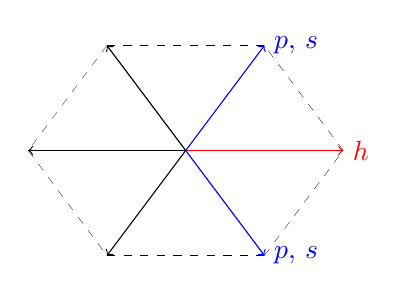
\begin{tikzpicture}
\draw[->, thin, red] (0, 0)--(2,0) node[right]{$h$};
\draw[->, thin, blue] (0, 0)--(1,-4/3) node[right]{$p, \, s$};
\draw[->, thin, blue] (0, 0)--(1,4/3) node[right]{$p, \, s$};
\draw[->, thin] (0, 0)--(-2,0);
\draw[->, thin] (0, 0)--(-1,-4/3);
\draw[->, thin] (0, 0)--(-1,4/3);

\draw[dashed, ultra thin] (2, 0)--(1, 4/3);
\draw[dashed, ultra thin] (1, 4/3)--(-1, 4/3);
\draw[dashed, ultra thin] (-1, 4/3)--(-2, 0);
\draw[dashed, ultra thin] (-2, 0)--(-1, -4/3);
\draw[dashed, ultra thin] (-1, -4/3)--(1,- 4/3);
\draw[dashed, ultra thin] (1, -4/3)--(2, 0);
\end{tikzpicture}
          }
         }
         \caption{The Lie algebra $\mathrm{su}(3, \, \C)$.}
\end{figure}

\begin{figure}[h!]
 \centering{   
\scalebox{.8}{ 
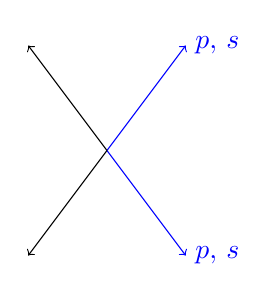
\begin{tikzpicture}
\draw[->, thin, blue] (0, 0)--(1,-4/3) node[right]{$p, \, s$};
\draw[->, thin, blue] (0, 0)--(1,4/3) node[right]{$p, \, s$};
\draw[->, thin] (0, 0)--(-1,-4/3);
\draw[->, thin] (0, 0)--(-1,4/3);
\end{tikzpicture}
          }
         }
         \caption{The Lie algebra $\mathrm{so}(4, \, \R) \sim \mathrm{su}(2, \, \C) \times \mathrm{su}(2, \, \C)$.}
\end{figure}

\begin{figure}[h!]
  \centering
        \mbox{%
\begin{minipage}{.30\textwidth}
\scalebox{.8}{ 
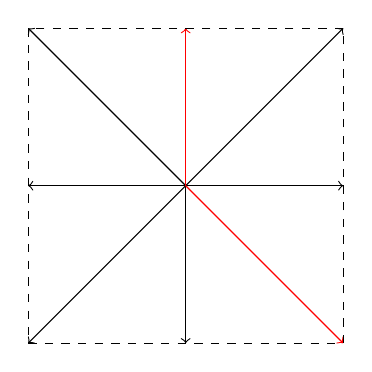
\begin{tikzpicture}
\draw[->, thin] (0, 0)--(2,0);
\draw[->, thin] (0, 0)--(0,-2);
\draw[->, thin] (0, 0)--(-2,0);
\draw[->, thin] (0, 0)--(2, 2);
\draw[->, thin] (0, 0)--(-2, 2);
\draw[->, thin] (0, 0)--(-2, -2);
\draw[->, thin, red] (0, 0)--(0,2);
\draw[->, thin, red] (0, 0)--(2, -2);

\draw[dashed, ultra thin] (2, 2)--(-2,2);
\draw[dashed, ultra thin] (-2, 2)--(-2, -2);
\draw[dashed, ultra thin] (-2, -2)--(2,-2);
\draw[dashed, ultra thin] (2, -2)--(2,2);
\end{tikzpicture}
          }
          \end{minipage}%
          \qquad \qquad
         \begin{minipage}{.30\textwidth}
\scalebox{.8}{ 
\begin{tikzpicture}
\draw[->, thin] (0, 0)--(2,0);
\draw[->, thin] (0, 0)--(0,-2);
\draw[->, thin] (0, 0)--(-2,0);
\draw[->, thin] (0, 0)--(1,1);
\draw[->, thin] (0, 0)--(-1, 1);
\draw[->, thin] (0, 0)--(-1, -1);
\draw[->, thin, red] (0, 0)--(0,2);
\draw[->, thin, red] (0, 0)--(1, -1);

\draw[dashed, ultra thin] (2, 0)--(0,2);
\draw[dashed, ultra thin] (0, 2)--(-2, 0);
\draw[dashed, ultra thin] (-2, 0)--(0,-2);
\draw[dashed, ultra thin] (0, -2)--(2,0);
\end{tikzpicture}
          }
          \end{minipage}%

         }
         \caption{The Lie algebras $\mathrm{so}(5, \, \R)$ and $\mathrm{usp}(4, \, \C)$. The color {\color{red}red} denotes the two simple roots. }
\end{figure}

\section{Dynkin Diagram} \index{Dynkin diagram}

The $2$-dimensional Dynkin diagram is a valuable tool to picture the rank-two algebras studied above, without relying on the weight diagram. We introduce the following notation: \mbox{}
\begin{enumerate}[label=\textbf{(\arabic*)}]
\item We denote by $\circ$ the bigger simple root, and by $\bullet$ the smaller simple root.
\item We denote the angle between $\alpha$ and $\beta$ simple roots with a number of segments equal to the number in the first column of \hyperref[table:1]{Figure 12.3}.
\end{enumerate}

The following Dynking Diagrams are an easy consequence of what we have proved so far in this chapter and, especially, in the last section.

\begin{equation*} \begin{aligned} & \mathrm{so}(4, \, \R) \: : \qquad
  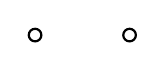
\begin{tikzpicture}[scale=.4]
    \draw[thick] (0, 0) circle (2 mm);
     \draw[thick] (3, 0) circle (2 mm);
  \end{tikzpicture}
  \\[1em] & \mathrm{su}(3, \, \C) \: : \qquad
  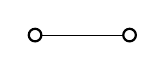
\begin{tikzpicture}[scale=.4]
    \draw[thick] (0, 0) circle (2 mm);
     \draw[thick] (3, 0) circle (2 mm);
     \draw[thin] (0.2, 0) -- (2.8,0);
  \end{tikzpicture}
    \\[1em] & \mathrm{su}(4, \, \C) \: : \qquad
  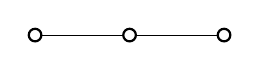
\begin{tikzpicture}[scale=.4]
    \draw[thick] (0, 0) circle (2 mm);
     \draw[thick] (3, 0) circle (2 mm);
     \draw[thick] (6, 0) circle (2mm);
     \draw[thin] (0.2, 0) -- (2.8,0);
     \draw[thin] (3.2, 0) -- (5.8,0);
  \end{tikzpicture}
     \\[1em] & \mathrm{su}(n + 1, \, \C) \: : \qquad
  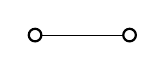
\begin{tikzpicture}[scale=.4]
    \draw[thick] (0, 0) circle (2 mm);
     \draw[thick] (3, 0) circle (2 mm);
     \draw[thin] (0.2, 0) -- (2.8,0);
  \end{tikzpicture} \dots 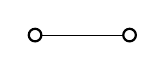
\begin{tikzpicture}[scale=.4]
    \draw[thick] (0, 0) circle (2 mm);
     \draw[thick] (3, 0) circle (2 mm);
     \draw[thin] (0.2, 0) -- (2.8,0);
  \end{tikzpicture} 
\end{aligned}\end{equation*}
We can also use the Dynking diagrams to show that $\mathrm{so}(5, \, \R)$ is isomorphic (as a Lie algebra) to $\mathrm{usp}(4, \, \C)$, and $\mathrm{su}(4, \, \C)$ is isomorphic to $\mathrm{so}(4, \, \R)$. Namely, we have
\begin{center}
  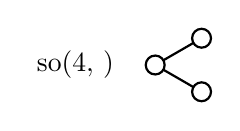
\begin{tikzpicture}[scale=.4]
    \draw (-1,0) node[anchor=east]  {$\mathrm{so}(4, \, \R)$};
  
    \draw[thick] (0 ,0) circle (.3 cm);
    \draw[thick] (30: 17 mm) circle (.3cm);
    \draw[thick] (-30: 17 mm) circle (.3cm);
    \draw[thick] (30: 3 mm) -- (30: 14 mm);
    \draw[thick] (-30: 3 mm) -- (-30: 14 mm);
  \end{tikzpicture}
\end{center}
which is clearly equivalent to $\mathrm{su}(4, \, \C)$. We also have
\begin{center}
  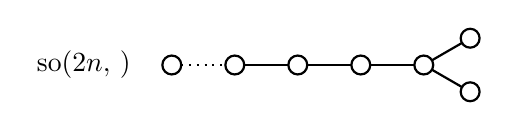
\begin{tikzpicture}[scale=.4]
    \draw (-1,0) node[anchor=east]  {$\mathrm{so}(2n, \, \R)$};
    \foreach \x in {0,...,4}
    \draw[xshift=\x cm,thick] (\x cm,0) circle (.3cm);
    \draw[xshift=8 cm,thick] (30: 17 mm) circle (.3cm);
    \draw[xshift=8 cm,thick] (-30: 17 mm) circle (.3cm);
    \draw[dotted,thick] (0.3 cm,0) -- +(1.4 cm,0);
    \foreach \y in {1.15,...,3.15}
    \draw[xshift=\y cm,thick] (\y cm,0) -- +(1.4 cm,0);
    \draw[xshift=8 cm,thick] (30: 3 mm) -- (30: 14 mm);
    \draw[xshift=8 cm,thick] (-30: 3 mm) -- (-30: 14 mm);
  \end{tikzpicture}
\end{center}
while, for odd natural numbers, we have
\begin{center}
  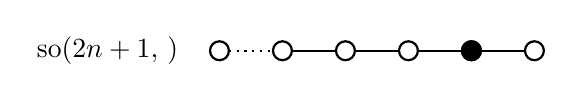
\begin{tikzpicture}[scale=.4]
    \draw (-1,0) node[anchor=east]  {$\mathrm{so}(2n + 1, \, \R)$};
    \foreach \x in {0,...,4}
    \draw[xshift=\x cm,thick] (\x cm,0) circle (.3cm);
    \draw[xshift=5 cm,thick,fill=white] (5 cm, 0) circle (.3 cm);
    \draw[dotted,thick] (0.3 cm,0) -- +(1.4 cm,0);
    \draw[xshift=5 cm,thick,fill=black] (3 cm, 0) circle (.3 cm);
    \foreach \y in {1.15,...,3.15}
    \draw[xshift=\y cm,thick] (\y cm,0) -- +(1.4 cm,0);
    \draw[thick] (8.3 cm, 0 cm) -- +(1.4 cm,0);
  \end{tikzpicture}
\end{center}
Since
\begin{center}
  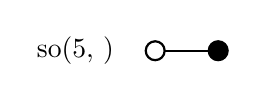
\begin{tikzpicture}[scale=.4]
    \draw (-1,0) node[anchor=east]  {$\mathrm{so}(5, \, \R)$};
    \draw[thick] (0 ,0) circle (.3 cm);
    \draw[thick,fill=black] (2 cm,0) circle (.3 cm);
    \draw[thick] (0: 3 mm) -- +(1.4 cm, 0);
  \end{tikzpicture}
\end{center}
and
\begin{center}
 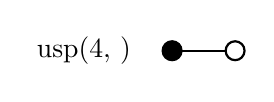
\begin{tikzpicture}[scale=.4]
    \draw (-1,0) node[anchor=east]  {$\mathrm{usp}(4, \, \C)$};
    \draw[thick, fill=black] (0 ,0) circle (.3 cm);
    \draw[thick,fill=white] (2 cm,0) circle (.3 cm);
    \draw[thick] (0: 3 mm) -- +(1.4 cm, 0);
  \end{tikzpicture}
\end{center}
we can easily infer that $\mathrm{so}(5, \, \R)$ is isomorphic (as a Lie algebra) to $\mathrm{usp}(4, \, \C)$.

{ \centering \subsubsection*{Dynking Diagram of Exceptional Groups} }

\begin{center}
  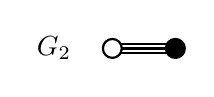
\begin{tikzpicture}[scale=.4]
    \draw (-1,0) node[anchor=east]  {$G_2$};
    \draw[thick] (0 ,0) circle (.3 cm);
    \draw[thick,fill=black] (2 cm,0) circle (.3 cm);
    \draw[thick] (30: 3mm) -- +(1.5 cm, 0);
    \draw[thick] (0: 3 mm) -- +(1.4 cm, 0);
    \draw[thick] (-30: 3 mm) -- +(1.5 cm, 0);
  \end{tikzpicture}
\end{center}

\begin{center}
  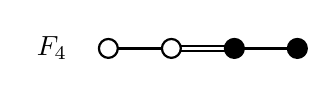
\begin{tikzpicture}[scale=.4]
    \draw (-3,0) node[anchor=east]  {$F_4$};
    \draw[thick] (-2 cm ,0) circle (.3 cm);
    \draw[thick] (0 ,0) circle (.3 cm);
    \draw[thick,fill=black] (2 cm,0) circle (.3 cm);
    \draw[thick,fill=black] (4 cm,0) circle (.3 cm);
    \draw[thick] (15: 3mm) -- +(1.5 cm, 0);
    \draw[xshift=-2 cm,thick] (0: 3 mm) -- +(1.4 cm, 0);
    \draw[thick] (-15: 3 mm) -- +(1.5 cm, 0);
    \draw[xshift=2 cm,thick] (0: 3 mm) -- +(1.4 cm, 0);
  \end{tikzpicture}
\end{center}

\begin{center}
  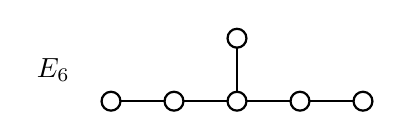
\begin{tikzpicture}[scale=.4]
    \draw (-1,1) node[anchor=east]  {$E_6$};
    \foreach \x in {0,...,4}
    \draw[thick,xshift=\x cm] (\x cm,0) circle (3 mm);
    \foreach \y in {0,...,3}
    \draw[thick,xshift=\y cm] (\y cm,0) ++(.3 cm, 0) -- +(14 mm,0);
    \draw[thick] (4 cm,2 cm) circle (3 mm);
    \draw[thick] (4 cm, 3mm) -- +(0, 1.4 cm);
  \end{tikzpicture}
\end{center}

\begin{center}
  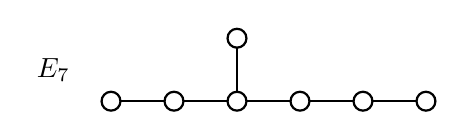
\begin{tikzpicture}[scale=.4]
    \draw (-1,1) node[anchor=east]  {$E_7$};
    \foreach \x in {0,...,5}
    \draw[thick,xshift=\x cm] (\x cm,0) circle (3 mm);
    \foreach \y in {0,...,4}
    \draw[thick,xshift=\y cm] (\y cm,0) ++(.3 cm, 0) -- +(14 mm,0);
    \draw[thick] (4 cm,2 cm) circle (3 mm);
    \draw[thick] (4 cm, 3mm) -- +(0, 1.4 cm);
  \end{tikzpicture}
\end{center}

\begin{center}
  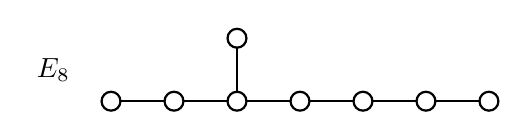
\begin{tikzpicture}[scale=.4]
    \draw (-1,1) node[anchor=east]  {$E_8$};
    \foreach \x in {0,...,6}
    \draw[thick,xshift=\x cm] (\x cm,0) circle (3 mm);
    \foreach \y in {0,...,5}
    \draw[thick,xshift=\y cm] (\y cm,0) ++(.3 cm, 0) -- +(14 mm,0);
    \draw[thick] (4 cm,2 cm) circle (3 mm);
    \draw[thick] (4 cm, 3mm) -- +(0, 1.4 cm);
  \end{tikzpicture}
\end{center}

\section{Cartan Matrices} \index{Cartan matrix}

Let $\mathfrak{L}$ be the set of simple roots of a semisimple Lie algebra $\g$. The \textit{Cartan matrix} is defined \caution{The non-diagonal elements of the Cartan matrix represent the angles between the simple roots of $\g$.}by setting
\begin{equation*} (A^\g)_{i, \, j} := 2 \frac{\alpha_i \alpha_j}{\alpha_i^2} \quad \text{for $i, \, j \in \{1, \, \dots, \, m \}$}, \end{equation*}
where $m$ is the rank of $\g$. 

\begin{example} In the case of $\mathrm{su}(3, \, \C)$, the matrix is given by
\begin{equation*} A = \begin{pmatrix} 2 & - 1\\-1 & 2 \end{pmatrix}. \end{equation*}
 \end{example}
 
 \begin{example} In the case of $\mathrm{su}(4, \, \C)$, the matrix is given by
\begin{equation*} A = \begin{pmatrix} 2 & - 1 & 0 \\-1 & 2 & - 1 \\ 0 & - 1 & 2\end{pmatrix}. \end{equation*}
 \end{example}
 
{\centering \subsubsection*{The construction of the Lie algebra $\mathrm{su}(3, \, \C)$}}

The simple roots of $\mathrm{su}(3, \, \C)$ are
\begin{equation*} \alpha_1 = \left( \frac{1}{2}, \, \frac{\sqrt{3}}{2} \right) \quad \text{and} \quad \alpha_2 = \left( \frac{1}{2}, \, - \frac{\sqrt{3}}{2} \right) \end{equation*}
and we have already proved that $\alpha_1 + \alpha_2$ is also a root. It is easy to check that
\begin{equation*} \frac{ \alpha_1 \cdot \alpha_2 }{\alpha_1^2} = - \frac{1}{2} \implies J_{\alpha_1}^3 \, | \, \alpha_2 \rangle = - \frac{1}{2} \, | \, \alpha_2 \rangle, \end{equation*}
and therefore $- j = 1/2$. We are now ready to show the construction of the Lie algebra:
\begin{equation*}\begin{aligned} [E_{\alpha_1}, \, E_{\alpha_2}] &= (T^{\alpha_1})_{\beta \alpha_2} E_\beta =
\\[1em] & = \langle \beta \, | \, T^{\alpha_1} \, | \, \alpha_2 \rangle E_\beta =
\\[1em] & = \langle \beta \, | \, J_1^{\alpha_1} \, | \, \alpha_2 \rangle E_\beta =
\\[1em] & = \frac{1}{\sqrt{2}} E_{\alpha_1 + \alpha_2}. \end{aligned}  \end{equation*}
Using this relation and the Jacobi identity \eqref{jacobi}, we infer that
\begin{equation*}\begin{aligned} [E_{-\alpha_1}, \, E_{\alpha_1 + \alpha_2}] &= \sqrt{2} \left[E_{-\alpha_1}, \, [E_{\alpha_1}, \, E_{\alpha_2}] \right] =
\\[1em] & = - \sqrt{2} \left[E_{\alpha_1}, \, \underbracket{[E_{\alpha_2}, \, E_{-\alpha_1}]}_{= 0} \right] - \sqrt{2} \left[E_{\alpha_2}, \, [E_{-\alpha_1}, \, E_{\alpha_1}] \right]  =
\\[1em] & = \sqrt{2} [ \alpha_1 \cdot \mathbf{H}, \, E_{\alpha_2} ] =
\\[1em] & = - \sqrt{2} \alpha_1 \cdot \alpha_2 E_{\alpha_2} = \frac{1}{\sqrt{2}} E_{\alpha_2}. \end{aligned}  \end{equation*}
In a similar fashion, one can prove that
\begin{equation*}\begin{aligned} [E_{-\alpha_2}, \, E_{\alpha_1 + \alpha_2}] &= \sqrt{2} \left[E_{-\alpha_2}, \, [E_{\alpha_1}, \, E_{\alpha_2}] \right] =
\\[1em] & = - \sqrt{2} \left[E_{\alpha_1}, \, [E_{\alpha_2}, \, E_{-\alpha_2}] \right] - \sqrt{2} \left[E_{\alpha_2}, \, \underbracket{[E_{-\alpha_2}, \, E_{\alpha_1}]}_{= 0} \right]  =
\\[1em] & = -\sqrt{2} [E_{\alpha_1}, \, \alpha_2 \cdot \mathbf{H} ] =
\\[1em] & = \sqrt{2} \alpha_1 \cdot \alpha_2 E_{\alpha_1} = - \frac{1}{\sqrt{2}} E_{\alpha_1}. \end{aligned}  \end{equation*}
In particular, the coefficients $N_{\alpha \beta}$ of \eqref{eq.f.1} have been entirely determined, and it is not hard to see that this is the Lie algebra $\mathrm{su}(3, \, \C)$.

\subsection{Weyl Reflection Group} \index{Weyl reflection group}

Let $\alpha, \, \beta \in \Delta$ be roots. We have proved in \hyperref[thm.f.1]{Theorem \ref{thm.f.1}} that the Weyl reflection, given by
\begin{equation*} \beta - \frac{2 \alpha( \alpha \cdot \beta)}{\alpha \cdot \alpha}, \end{equation*}
is also a root. The set of Weyl reflections preserves the weights diagram, as one can easily check by computing the action of the operators $J_\alpha^i$ against $\beta$.

\begin{theorem}The trace of any generator of any representation of a compact simple Lie group is zero \end{theorem}

\begin{proof}See \cite{alsd} for a detailed dissertation on the topic. \end{proof}